\documentclass[a4paper]{article}
\usepackage{color}              %Farben, f.r \definecolor{}
\usepackage{amssymb}            %Mathematische Symbole
\usepackage{amsthm}             %Besseres \newtheorem
\usepackage{amsmath}           %Mathematische Umgebungen
\usepackage{mathtools}          %\xRightarrow, etc
\usepackage{mathrsfs}           %enthaelt \mathscr
\usepackage{graphicx}
\usepackage{enumerate}          % in-place numerations def.
\usepackage{fullpage}

\usepackage{array}
%\usepackage{multicol}
%\usepackage[notref,notcite]{showkeys}
%\usepackage{algorithm,algorithmic}
\usepackage{color}

\usepackage{graphicx}
\usepackage{xypic}
\entrymodifiers={+!!<0pt,\fontdimen22\textfont2>}
\usepackage[all]{xy}

\usepackage{float}
\usepackage{tikz}
\usepackage{tikz-cd}
\usepackage{tikz,fullpage}
\usetikzlibrary{arrows,%
                petri,%
                topaths}%
\usepackage{tkz-berge}
\usepackage[position=top]{subfig}
\usetikzlibrary{shapes.geometric}
\usetikzlibrary{decorations.markings}

\newtheoremstyle{myremark} % name
    {7pt}                    % Space above
    {7pt}                    % Space below
    {}  	                 % Body font
    {}                           % Indent amount
    {\bf}       	         % Theorem head font
    {.}                          % Punctuation after theorem head
    {.5em}                       % Space after theorem head
    {}  % Theorem head spec (can be left empty, meaning ‘normal’)

\theoremstyle{plain}
\newtheorem{lemma}{Lemma}
\newtheorem{theorem}[lemma]{Theorem}
\newtheorem{fact}[lemma]{Fact}
\newtheorem{definition}[lemma]{Definition}
\newtheorem{corollary}[lemma]{Corollary}
\newtheorem{proposition}[lemma]{Proposition}
\newtheorem{conjecture}[lemma]{Conjecture}
\newtheorem{observation}[lemma]{Observation}
\newtheorem{problem}[lemma]{Problem}
\newtheorem{notation}[lemma]{Notation}
\newtheorem*{claim}{Claim}

\theoremstyle{myremark}
\newtheorem{remark}[lemma]{Remark}
\newtheorem{example}[lemma]{Example}
\newtheorem{exercise}[lemma]{Exercise}
\newtheorem{algorithm}[lemma]{Algorithm}
\newtheorem{application}[lemma]{Application}
\newtheorem*{goal}{Goal}

%%%%%% EDIT HERE: %%%%%%%%%%%
\newcommand{\LECTURENUMBER}{0}
\newcommand{\LECTURETITLE}{Short title}
\newcommand{\LECTURESCRIBE}{Your name}

%% Dokument Beginn %%%%%%%%%%%%%%%%%%%%%%%%%%%%%%%%%%%%%%%%%%%%%%%%%%%%%%%%
\begin{document}
\thispagestyle{empty}

\begin{center}
	{\Large\bf Graph coloring}\\
	{\bf Lecture notes, vol. 2 \\ Basics of graph theory and coloring}\\
\end{center}
Lecturer: Michal Adamaszek \hfill Scribe: Giorgia L. G. Cassis
\begin{center}
\line(1,0){450}
\end{center}

%%%%%%% EDIT ALSO BELOW: %%%%%%%%%%%%%%%%

In the next pages, $G$ is always a graph, $V(G)$ its set of vertices and $E(G)$ its set of edges. 
\begin{definition}
A \emph{walk} in $G$ from $u$ to $v$ ($u,v, \in V(G)$) is a sequence
$$u=x_1,x_2,\dots,x_k=v,$$
such that $x_ix_{i+1} \in E(G)$ for all $i$. This walk is called closed if $u=v$. Moreover:
\begin{enumerate}
\item $G$ s called \emph{connected} if there is a walk between any two vertices,
\item $G$ is called \emph{disconnected} otherwise.
\end{enumerate}
\end{definition}

\begin{definition} The \emph{distance} between $u$ and $v$ ($u,v, \in V(G)$) is
$$d(u,v):=
\begin{cases} 
\text{length of the shortest walk from $u$ to $v$}, & \text{if $\exists$ a walk between $u$ and $v$}\\ 
\infty, & \text{if $\nexists$ a walk between $u$ and $v$}\\
0, & \text{if } u=v
\end{cases}.$$
Moreover the \emph{diameter} of $G$ is
$$diam(G):= \max_{u,v\in V(G)}(d(u,v)).$$
\end{definition}

\begin{exercise} In the definition of connectedness and distance we can replace \emph{walk} with \emph{path}.
\end{exercise}

\begin{lemma} $G$ is disconnected $\Longleftrightarrow \exists$ non-empty sets $X,Y$ with $V(G)=X \cup Y$, $X \cap Y=\emptyset$ such that there is no edge from $X$ to $Y$.
\end{lemma}

\begin{proof}
\emph{$(\Leftarrow)$} Take $u\in X$ and $v \in Y$, then clearly $d(u,v)=\infty$ and $G$ is disconnected.
\\ \emph{$(\Rightarrow)$} If $G$ is disconnected, then we can find $u,v\in V(G)$ with $d(u,v)=\infty$. We define
$$X:=\{x\in V(G): \ d(u,x)<\infty \},$$
$$Y:=V(G) \backslash X.$$
Since $u\in X$ and $v\in Y$, these two sets are non-empty. Moreover there is no edge between these two sets: assume there exist $w\in X,\ z\in Y$ such that $wz \in E(G)$, then $d(u,z)\leqslant d(u,w)+1 <\infty$, which is a contradiction.

\begin{figure}[H]
\begin{center}
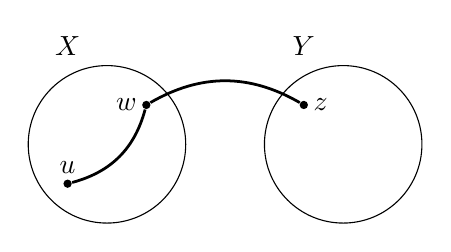
\begin{tikzpicture} 
\draw (-1.5,0) circle (1) (-2,1)  node [text=black,above] {$X$}
      (1.5,0) circle (1) (1,1)  node [text=black,above] {$Y$};

\draw  node[fill,circle,inner sep=0pt,minimum size=3pt] (n1) at (-2,-0.5) {} 
(-2, -0.5) node [text=black,above] {$u$}
 
	node[fill,circle,inner sep=0pt,minimum size=3pt] (n2) at (-1,0.5) {}
(-1,0.5) node [text=black,left] {$w$}

	node[fill,circle,inner sep=0pt,minimum size=3pt] (n3) at (1,0.5) {}
(1,0.5) node [text=black,right] {$z$};

\draw [line width = 1 pt, black, -, bend right] (n1) edge node {} (n2)
	[line width = 1 pt, black, -, bend left] (n2) edge node {} (n3);
\end{tikzpicture}
\end{center}
\end{figure}
\end{proof}

\section*{Trees}
\begin{definition} A \emph{tree} is a connected graph without cycles. A \emph{forest} is a graph, whose every connected component is a tree.
\begin{figure}[H]
\begin{center}
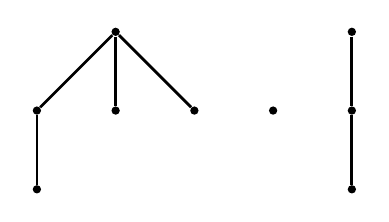
\begin{tikzpicture} 
\draw  node[fill,circle,inner sep=0pt,minimum size=3pt] (n1) at (0,0) {}
	node[fill,circle,inner sep=0pt,minimum size=3pt] (n2) at (-1,-1) {}
		node[fill,circle,inner sep=0pt,minimum size=3pt] (n3) at (0,-1) {} 
	node[fill,circle,inner sep=0pt,minimum size=3pt] (n4) at (1,-1) {} 
	node[fill,circle,inner sep=0pt,minimum size=3pt] (n5) at (-1,-2) {}
	node[fill,circle,inner sep=0pt,minimum size=3pt] (n6) at (2,-1) {}
	node[fill,circle,inner sep=0pt,minimum size=3pt] (n7) at (3,0) {}
	node[fill,circle,inner sep=0pt,minimum size=3pt] (n8) at (3,-1) {}
	node[fill,circle,inner sep=0pt,minimum size=3pt] (n9) at (3,-2) {};
	
\draw [line width = 1 pt, black, -] (n1) edge node {} (n2)
[line width = 1 pt, black, -] (n1) edge node {} (n3)
[line width = 1 pt, black, -] (n1) edge node {} (n4)
[line width = 1 pt, black, -] (n2) edge node {} (n5)
[line width = 1 pt, black, -] (n8) edge node {} (n9)
[line width = 1 pt, black, -] (n7) edge node {} (n8);
\end{tikzpicture}
\end{center}
\end{figure}
\end{definition}

\begin{theorem} The following are equivalent:
\begin{enumerate}
\item $G$ is a tree,
\item $G$ is connected and $|E(G)|=|V(G)|-1$,
\item Every two vertices of $G$ are connected by exactly one path.
\end{enumerate}
\end{theorem}

\begin{proof}
\emph{$(3\Rightarrow 1)$} $G$ is already connected by assumption, hence we must only show that $G$ has no cycles. Assume that we an find one, then all vertices $u,v$ from that cycle are connected by $\geqslant 2$ paths, which is a contradiction.
\\ \emph{$(1\Rightarrow 2)$} We work with induction on the number of vertices (let $|V(G)|=n$). For $n=1$ we clearly have no edges. Assume $n\geqslant 2$. Since $G$ is connected we can choose an edge $e\in E(G)$. Let us take a look at $G-e$ ($G$ without $e$):
\begin{figure}[H]
\begin{center}
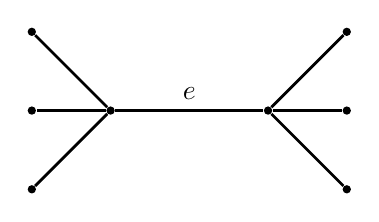
\begin{tikzpicture} 
\draw  node[fill,circle,inner sep=0pt,minimum size=3pt] (n1) at (-1,0) {}
	node[fill,circle,inner sep=0pt,minimum size=3pt] (n2) at (1,0) {}
		node[fill,circle,inner sep=0pt,minimum size=3pt] (n3) at (-2,1) {} 
	node[fill,circle,inner sep=0pt,minimum size=3pt] (n4) at (-2,0) {} 
	node[fill,circle,inner sep=0pt,minimum size=3pt] (n5) at (-2,-1) {}
	node[fill,circle,inner sep=0pt,minimum size=3pt] (n6) at (2,1) {}
	node[fill,circle,inner sep=0pt,minimum size=3pt] (n7) at (2,0) {}
	node[fill,circle,inner sep=0pt,minimum size=3pt] (n8) at (2,-1) {};
	
\draw [line width = 1 pt, black, -] (n1) edge node {} (n2) (0,0) node [above] {$e$}
[line width = 1 pt, black, -] (n1) edge node {} (n3)
[line width = 1 pt, black, -] (n1) edge node {} (n4)
[line width = 1 pt, black, -] (n1) edge node {} (n5)
[line width = 1 pt, black, -] (n2) edge node {} (n6)
[line width = 1 pt, black, -] (n2) edge node {} (n7)
[line width = 1 pt, black, -] (n2) edge node {} (n8);
\end{tikzpicture}
\end{center}
\end{figure}
Removing an edge generates at most $2$ connected components (call them $G_1$ and $G_2$), both without cycles. Since $G$ was a tree, $G_1$ and $G_2$ are connected and $G-e$ is a forest with two components. We can compute
\begin{align*}
|E(G)|&=1+|E(G_1)|+|E(G_2)|\overbrace{=}^{\text{i.a.}}1+|V(G_1)|-1+|V(G_2)|-1=\\
&=|V(G_1)|+|V(G_2)|-1 = |V(G)|-1.
\end{align*}

\emph{$(2\Rightarrow 3)$} Assume we already proved Lemma \ref{Lemma 7}, then we can find a leaf $v\in V(G)$. Let $w$ be the only neighbour of $v$. $G-v$ is again connected and we have
$$|E(G-v)|=|V(G-v)|-1.$$
Working with induction (whose initial step is obvious) we can say that every two vertices in $G-v$ are connected by exactly one path, hence there is also a unique path $x,w,v$ for every $x\in V(G-v)$.
\end{proof}

\begin{lemma} \label{Lemma 7}
Any tree has at least $2$ leaves, provided that it has at least $2$ vertices.
\end{lemma}

\begin{proof}
Let $G$ be a tree with $n$ vertices and $n-1$ edges. Since $G$ is connected, then 
$$\forall v\in V(G): \ deg(v)\geqslant 1.$$
Suppose that we only have $1$ leaf, then
$$\underbrace{2(n-1)}_{\substack{\text{all other vertices}\\ \text{have degree} \geqslant 2}} +\underbrace{1}_{\text{leaf}} \leqslant \sum_{v\in V(G)}deg(v)=2(n-1),$$
which is a contradiction. The same follows if we allow no leaves.
\end{proof}

\section*{Bipartite graphs}
\begin{definition} $G$ is \emph{bipartite} if there are two sets $A$ and $B$ with $V(G)=A\cup B$, $A\cap B=\emptyset$ such that every edge of $G$ has one end in each part.
\end{definition}

\begin{example} We can use bipartite graph to illustrate a scheduling problem.
\begin{figure}[H]
\begin{center}
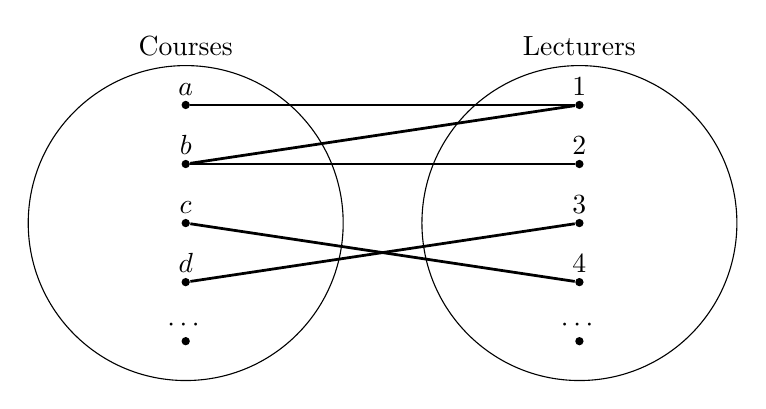
\begin{tikzpicture} 
\draw (-2.5,0) circle (2) (-2.5,2)  node [text=black,above] {Courses}
      (2.5,0) circle (2) (2.5,2)  node [text=black,above] {Lecturers};

\draw  node[fill,circle,inner sep=0pt,minimum size=3pt] (n1) at (-2.5,1.5) {} 
(-2.5,1.5) node [text=black,above] {$a$}
	node[fill,circle,inner sep=0pt,minimum size=3pt] (n2) at (-2.5,0.75) {} 
(-2.5,0.75) node [text=black,above] {$b$}
	node[fill,circle,inner sep=0pt,minimum size=3pt] (n3) at (-2.5,0) {} 
(-2.5,0) node [text=black,above] {$c$}
	node[fill,circle,inner sep=0pt,minimum size=3pt] (n4) at (-2.5,-0.75) {} 
(-2.5,-0.75) node [text=black,above] {$d$}
	node[fill,circle,inner sep=0pt,minimum size=3pt] (n5) at (-2.5,-1.5) {} 
(-2.5,-1.5) node [text=black,above] {$\cdots$}

	node[fill,circle,inner sep=0pt,minimum size=3pt] (n6) at (2.5,1.5) {} 
(2.5,1.5) node [text=black,above] {$1$}
	node[fill,circle,inner sep=0pt,minimum size=3pt] (n7) at (2.5,0.75) {} 
(2.5,0.75) node [text=black,above] {$2$}
	node[fill,circle,inner sep=0pt,minimum size=3pt] (n8) at (2.5,0) {} 
(2.5,0) node [text=black,above] {$3$}
	node[fill,circle,inner sep=0pt,minimum size=3pt] (n9) at (2.5,-0.75) {} 
(2.5,-0.75) node [text=black,above] {$4$}
	node[fill,circle,inner sep=0pt,minimum size=3pt] (n10) at (2.5,-1.5) {} 
(2.5,-1.5) node [text=black,above] {$\cdots$};

\draw [line width = 1 pt, black, -] (n6) edge node {} (n1)
 	[line width = 1 pt, black, -] (n6) edge node {} (n2)
 	 [line width = 1 pt, black, -] (n7) edge node {} (n2)
  	 [line width = 1 pt, black, -] (n8) edge node {} (n4)
 	 [line width = 1 pt, black, -] (n9) edge node {} (n3);
\end{tikzpicture}
\end{center}
\end{figure}
\end{example}

\begin{example}
\begin{itemize}
\item Complete bipartite graphs ($K_{n,m}$): two sets $A$ and $B$ (with $|A|=n$ and $|B|=m$) with all the possible edges in between.
\item Trees: 
\begin{figure}[H]
\begin{center}
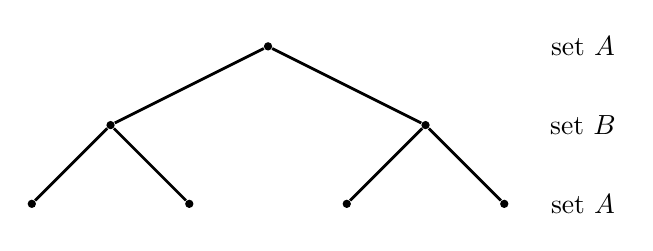
\begin{tikzpicture} 
\draw  node[fill,circle,inner sep=0pt,minimum size=3pt] (n1) at (0,0) {} 
	node[fill,circle,inner sep=0pt,minimum size=3pt] (n2) at (-2,-1) {} 
	node[fill,circle,inner sep=0pt,minimum size=3pt] (n3) at (2,-1) {} 
	node[fill,circle,inner sep=0pt,minimum size=3pt] (n4) at (-3,-2) {} 
	node[fill,circle,inner sep=0pt,minimum size=3pt] (n5) at (-1,-2) {} 
	node[fill,circle,inner sep=0pt,minimum size=3pt] (n6) at (1,-2) {} 
	node[fill,circle,inner sep=0pt,minimum size=3pt] (n7) at (3,-2) {} 

(4,0) node [text=black] {\text{set} $A$}			
(4,-1) node [text=black] {\text{set} $B$} 
(4,-2) node [text=black] {\text{set} $A$};

\draw [line width = 1 pt, black, -] (n1) edge node {} (n2)
 	[line width = 1 pt, black, -] (n1) edge node {} (n3)
 	 [line width = 1 pt, black, -] (n2) edge node {} (n4)
  	 [line width = 1 pt, black, -] (n2) edge node {} (n5)
 	 [line width = 1 pt, black, -] (n3) edge node {} (n6)
   	 [line width = 1 pt, black, -] (n3) edge node {} (n7);
\end{tikzpicture}
\end{center}
\end{figure}
\item $n$-cubes graphs ($Q_n$): $V_n:=\{(x_1,\dots,x_n): \ x_i \in \{0,1\}\}$ and then define 
$$A_n:=\{(x_1,\dots,x_n) \in V_n: 2 \mid \sum_{i=1}^n x_i\},$$
$$B_n:=\{(x_1,\dots,x_n) \in V_n: 2 \not| \ \sum_{i=1}^n x_i\}.$$
Moving on one edge clearly changes the parity of the sequence, hence $V_n=A_n\cup B_n$ defines a bipartite graph.
\item Cycles: $C_{2n}$ is bipartite, $C_{2n+1}$ is not bipartite (for $n\in \mathbb{N}$).
\end{itemize}
\end{example}

\begin{theorem} \emph{(K\"{o}nig)}
$G$ is bipartite iff there is no closed walk of odd length.
\end{theorem}

\begin{proof}
\emph{$(\Leftarrow)$} If we start in $A$, after an odd number of steps we will be in $B$ (since each step brings to the other side of the graph).
\\ \emph{$(\Rightarrow)$} Assume that $G$ is connected (if not, work separately in each connected component). Pick $v\in V(G)$ and define
$$A:=\{w\in V(G): \exists \text{ an even-length walk } v\rightarrow w\},$$
$$B:=\{w\in V(G): \exists \text{ an odd-length walk } v\rightarrow w\}.$$
\begin{itemize}
\item $A\cup B=V(G)$, since $G$ is connected.
\item $A\cap B=\emptyset$, since otherwise we could find the following situation for a $w\in A\cap B$:
\begin{figure}[H]
\begin{center}
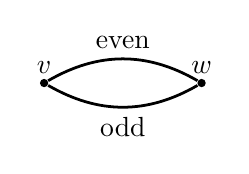
\begin{tikzpicture} 
\draw node[fill,circle,inner sep=0pt,minimum size=3pt] (n1) at (-1,0) {} 
(-1,0) node [text=black,above] {$v$}
	node[fill,circle,inner sep=0pt,minimum size=3pt] (n2) at (1,0) {} 
(1,0) node [text=black,above] {$w$};

\draw [line width = 1 pt, black, -, bend right] (n1) edge node {} (n2) (0,0.3) node [above] {even}
	[line width = 1 pt, black, -, bend left] (n1) edge node {} (n2) (0,-0.3) node [below] {odd};
\end{tikzpicture}
\end{center}
\end{figure}
This means we would have an odd closed walk.
\item There is no edge between two vertices in $A$ (resp. $B$), otherwise we would have the following situation:
\begin{figure}[H]
\begin{center}
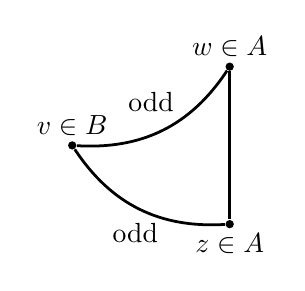
\begin{tikzpicture} 
\draw node[fill,circle,inner sep=0pt,minimum size=3pt] (n1) at (-1,0) {} 
(-1,0) node [text=black,above] {$v\in B$}
	node[fill,circle,inner sep=0pt,minimum size=3pt] (n2) at (1,1) {} 
(1,1) node [text=black,above] {$w\in A$}
	node[fill,circle,inner sep=0pt,minimum size=3pt] (n3) at (1,-1) {} 
(1,-1) node [text=black,below] {$z\in A$};

\draw 	[line width = 1 pt, black, -] (n2) edge node {} (n3)
	[line width = 1 pt, black, -, bend right] (n1) edge node {} (n2) (0,0.3) node [above] {odd}
	[line width = 1 pt, black, -, bend right] (n1) edge node {} (n3) (-0.2,-0.85) node [below] {odd};
\end{tikzpicture}
\end{center}
\end{figure}
\end{itemize}
\end{proof}

\begin{exercise}
In K\"{o}nig's theorem we can replace \emph{closed walk} with \emph{cycle} (and even \emph{induced cycle}).
\end{exercise}

\section*{Cliques and independent sets}
\begin{definition}
\begin{itemize}
\item $W\subseteq V(G)$ is a \emph{clique} if for all $x,y\in W$, $x\neq y$, we have $xy\in E(G)$,
\item $W\subseteq V(G)$ is an \emph{independent set} if for all $x,y\in W, \ xy\notin E(G)$.
\end{itemize}
\end{definition}

\begin{remark} A clique is a subgraph that is a complete graph.
\end{remark}

\begin{example} The followings are examples of cliques.
\begin{figure}[H]
\begin{center}
\begin{tikzpicture} 
\draw  node[fill=purple,circle,inner sep=0pt,minimum size=3pt] (n1) at (-1.5,0) {}
	node[fill=orange,circle,inner sep=0pt,minimum size=3pt] (n2) at (1.5,0) {}
		node[fill=purple,circle,inner sep=0pt,minimum size=3pt] (n3) at (0,1.5) {} 
	node[fill=purple,circle,inner sep=0pt,minimum size=3pt] (n4) at (0,-1.5) {} 
	node[fill=blue,circle,inner sep=0pt,minimum size=3pt] (n5) at (3,1.5) {}
	node[fill=orange,circle,inner sep=0pt,minimum size=3pt] (n6) at (3,-1) {};

\draw [color=purple] (-1.5,0) -- (0,1.5) node {};
\draw [color=purple] (-1.5,0) -- (0,-1.5) node {};
\draw [color=purple] (0,1.5) -- (0,-1.5) node {};

\draw [color=black] (0,1.5) -- (1.5,0) node {};
\draw [color=black] (0,-1.5) -- (1.5,0) node {};
\draw [color=black] (0,1.5) -- (3,1.5) node {};

\draw [color=orange] (1.5,0) -- (3,-1) node {};
\end{tikzpicture}
\end{center}
\end{figure}
\end{example}

\begin{example} The followings are examples of independent sets.
\begin{figure}[H]
\begin{center}
\begin{tikzpicture} 
\draw  node[fill=purple,circle,inner sep=0pt,minimum size=3pt] (n1) at (-1.5,0) {}
	node[fill=purple,circle,inner sep=0pt,minimum size=3pt] (n2) at (1.5,0) {}
		node[fill=orange,circle,inner sep=0pt,minimum size=3pt] (n3) at (0,1.5) {} 
	node[fill=blue,circle,inner sep=0pt,minimum size=3pt] (n4) at (0,-1.5) {} 
	node[fill=purple,circle,inner sep=0pt,minimum size=3pt] (n5) at (3,1.5) {}
	node[fill=orange,circle,inner sep=0pt,minimum size=3pt] (n6) at (3,-1) {};
	
\draw [color=black] (-1.5,0) -- (0,1.5) node {};
\draw [color=black] (-1.5,0) -- (0,-1.5) node {};
\draw [color=black] (0,1.5) -- (0,-1.5) node {};

\draw [color=black] (0,1.5) -- (1.5,0) node {};
\draw [color=black] (0,-1.5) -- (1.5,0) node {};
\draw [color=black] (0,1.5) -- (3,1.5) node {};

\draw [color=black] (1.5,0) -- (3,-1) node {};
\end{tikzpicture}
\end{center}
\end{figure}
\end{example}

\begin{definition}
\begin{itemize}
\item The \emph{clique number} of $G$, $\omega(G)$, is the cardinality of the biggest clique in $G$,
\item The \emph{independence number} of $G$, $\alpha(G)$, is the cardinality of the biggest independent set in $G$.
\end{itemize}
\end{definition}

\begin{observation}
\begin{enumerate}
\item $\alpha(G)=\omega(\overline{G})$.
\begin{proof}
A clique in $G$ is an independent set in $\overline{G}$ and vice versa.
\end{proof}
\item If $G$ is bipartite, then $\omega(G)\leqslant 2$.
\begin{proof}
If there is a triangle, then two of the vertices have to be in the same part of the bipartite graph, which is impossible by definition.
\end{proof}
\item $\omega(G)\leqslant 2$ does not imply that $G$ is bipartite.
\begin{proof}
$C_5$ (which is not bipartite since it is an odd cycle) has $\omega(C_5)=2$.
\end{proof}
\end{enumerate}
\end{observation}

\begin{definition} Graphs with $\omega(G)\leqslant 2$ are usually called triangle-free.
\end{definition}

\begin{example}
\begin{itemize}
\item $\omega(C_n)=
\begin{cases} 
3, & \text{if } n=3\\ 
2, & \text{if } n\geqslant 4
\end{cases}.$
\item $\alpha(C_n)=
\begin{cases} 
\frac{n}{2}, & \text{if } 2\mid n\\ 
\frac{n-1}{2}, & \text{if } 2\not| \ n
\end{cases}.$
\item $G$ bipartite (i.e. $V(G)=A\cup B$), then $\alpha(G)\geqslant max\{|A|,|B|\}$.
\item $\omega(K_n)=n$ and $\alpha(K_n)=1$.
\end{itemize}
\end{example}

\begin{remark} $\alpha$ and $\omega$ are hard (meaning $NP$-hard) to compute.
\end{remark}

\begin{lemma}
$\alpha(G)\geqslant \frac{|V(G)|}{1+\Delta(G)}$.
\end{lemma}

\begin{proof} We must find an independent set of size at least $\frac{|V(G)|}{1+\Delta(G)}$ and we will work by induction in order to do that. Take an arbitrary vertex $v\in V(G)$ and consider the graph 
$$G':=G-v-N_G(V).$$
Clearly $\Delta(G')\leqslant \Delta(G)$. Using the induction assumption, $G'$ has an independent set $X$ of size at least
$$\frac{|V(G')|}{1+\Delta(G')}.$$
Consider $X\cup \{v\}$, which (by construction) is an independent set in $G$.
$$|X\cup \{v\}|=|X|+1\geqslant\frac{|V(G')|}{1+\Delta(G')}+1\geqslant \frac{|V(G)|-(1+\Delta(G))}{1+\Delta(G)}+1=\frac{|V(G)|}{1+\Delta(G)},$$
thanks to $\Delta(G')\leqslant \Delta(G)$ and considering that $1+\Delta(G)$ is the biggest number of vertices we can take away while defining $G'$.
\end{proof}

\begin{algorithm} (The greedy algorithm) The following loop iterates $\geqslant \frac{|V(G)|}{1+\Delta(G)}$ times.
\begin{enumerate}
\item Take $v\in V(G)$,
\item Remove $v$ and $N_G(v)$ (at most $1+\Delta(G)$ vertices),
\item Iterate using $G':=G-v-N_G(V)$.
\end{enumerate}
\end{algorithm}

\begin{lemma} If $f:G\longrightarrow H$ is a graph homomorphism, then $f^{-1}(v)$ is an independent set for all $v\in V(H)$.
\end{lemma}

\begin{proof}
Suppose that $x,y\in f^{-1}(v)$ and $xy\in E(G)$. Then, since $f$ is a graph homomorphism, we would have $f(x)f(y)\in E(H)$, which is impossible since $f(x)=f(y)=v$.
\end{proof}

\section*{Vertex colouring}
\begin{goal} Assign colours to the vertices of a graph, such that adjacent vertices have different colours (the problem is optimized by finding the minimal number of colours needed for this process).
\end{goal}

\begin{application}
\begin{enumerate}
\item Colouring a land-map, such that the countries that share a border have different colours. In this case the vertices represent the countries and we draw an edge whenever two countries share a border.
\item Scheduling the timetable for an exam session. In this case the vertices represent the different subjects offered and we draw an edge whenever there is at least a student following both courses. Minimizing the number of colours means programming the minimal number of exam-spots, such that each student can take all the exams he/she applied for.
\end{enumerate}
\end{application}

\begin{example} Take a graph $G$ with $81$ vertices forming a $9\times9$ grid, such that the following conditions are satisfied:
\begin{itemize}
\item Every row is a clique,
\item Every column is a clique,
\item If we divide the grid forming $9$ $3\times 3$ subgrids, each of these is a clique.
\end{itemize}
Then each possible colouring represents the solutions of a Sudoku.
\end{example}

\begin{definition} A \emph{(vertex-)colouring} of $G$ with colour set $C$ is a function
$$c:V(G)\longrightarrow C,$$
such that if $xy\in E(G)$, then $c(x)\neq c(y)$.
\end{definition}

\begin{definition} The \emph{chromatic number} $\chi(G)$ is the smallest number $k$ for which there is a colouring of $G$ with $k$ colours. If $\chi(G)\leqslant k$, then $G$ is called \emph{$k$-colourable}.
\end{definition}

\begin{definition} Each $c^{-1}(i)$ is called a \emph{color class}.
\end{definition}

\begin{example}
\begin{itemize}
\item $\chi(P_n)=2$,
\item $\chi(C_n)=
\begin{cases} 
2, & \text{if } 2\mid n\\ 
3, & \text{if } 2\not| \ n
\end{cases},$
\item $\chi(K_n)=n$,
\item $\chi(Q_n)=2$, since $Q_n$ is bipartite. Moreover, $\chi$ of every bipartite graph with at least one edge is $2$.
\end{itemize}
\end{example}

\begin{lemma}
\begin{enumerate}
\item $\chi(G)\leqslant |V(G)|$,
\item $\chi(G)=|V(G)| \Longleftrightarrow G$ is complete,
\item $\chi(G)=1 \Longleftrightarrow G \simeq \overline{K_n},$
\item $\chi(G)=2 \Longleftrightarrow G$ is bipartite and has at least one edge.
\end{enumerate}
\end{lemma}

\begin{proof}
\begin{enumerate}
\item $c: |V(G)| \longrightarrow  |V(G)|$ with $c(v)=v$ is a colouring with exactly $|V(G)|$ colours.
\item One direction is obvious. Let us assume $G$ is not complete, then we can find $x,y\in V(G)$ with $xy\notin E(G)$. Set $c(x)=c(y)$ and colour all the other $|V(G)|-2$ vertices with different colours: this is a colouring with $|V(G)|-1$ colours.
\item One direction is obvious. For the other look at $c:V(G)\longrightarrow \{1\}$ with $c(x)=c(y)$ for all $x,y\in V(G)$. This implies $xy\notin E(G)$ for all $x,y\in V(G)$, hence $G \simeq \overline{K_n}$.
\item One direction is obvious. For the other, if $\chi(G)=2$ then it suffices to define $A:=c^{-1}(1)$ and $B:=c^{-1}(2)$ to find the partition of the set $V(G)$.
\end{enumerate}
\end{proof}

\begin{remark}
Already determining whether $\chi(G)\leqslant 3$ or $\chi(G)\geqslant 4$ is hard.
\end{remark}
\end{document}




